% Created by tikzDevice version 0.12.6 on 2025-05-07 15:06:44
% !TEX encoding = UTF-8 Unicode
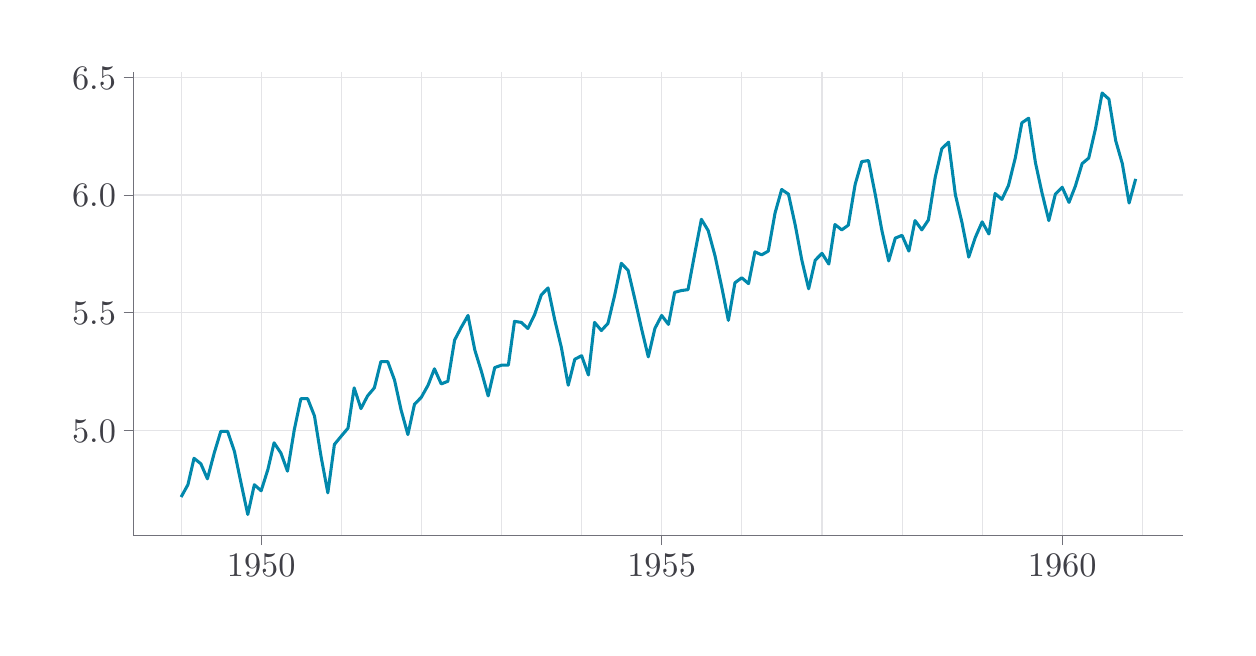
\begin{tikzpicture}[x=1pt,y=1pt]
\definecolor{fillColor}{RGB}{255,255,255}
\path[use as bounding box,fill=fillColor] (0,0) rectangle (433.62,216.81);
\begin{scope}
\path[clip] (  0.00,  0.00) rectangle (433.62,216.81);
\definecolor{drawColor}{RGB}{255,255,255}

\path[draw=drawColor,line width= 0.7pt,line join=round,line cap=round,fill=fillColor] (  0.00,  0.00) rectangle (433.62,216.81);
\end{scope}
\begin{scope}
\path[clip] ( 38.19, 33.29) rectangle (417.62,200.81);
\definecolor{drawColor}{RGB}{255,255,255}
\definecolor{fillColor}{RGB}{255,255,255}

\path[draw=drawColor,line width= 0.7pt,line join=round,line cap=round,fill=fillColor] ( 38.19, 33.29) rectangle (417.62,200.81);
\definecolor{drawColor}{RGB}{228,228,231}

\path[draw=drawColor,line width= 0.4pt,line join=round] ( 55.44, 33.29) --
	( 55.44,200.81);

\path[draw=drawColor,line width= 0.4pt,line join=round] (113.30, 33.29) --
	(113.30,200.81);

\path[draw=drawColor,line width= 0.4pt,line join=round] (142.23, 33.29) --
	(142.23,200.81);

\path[draw=drawColor,line width= 0.4pt,line join=round] (171.24, 33.29) --
	(171.24,200.81);

\path[draw=drawColor,line width= 0.4pt,line join=round] (200.17, 33.29) --
	(200.17,200.81);

\path[draw=drawColor,line width= 0.4pt,line join=round] (258.02, 33.29) --
	(258.02,200.81);

\path[draw=drawColor,line width= 0.4pt,line join=round] (287.03, 33.29) --
	(287.03,200.81);

\path[draw=drawColor,line width= 0.4pt,line join=round] (315.96, 33.29) --
	(315.96,200.81);

\path[draw=drawColor,line width= 0.4pt,line join=round] (344.89, 33.29) --
	(344.89,200.81);

\path[draw=drawColor,line width= 0.4pt,line join=round] (402.83, 33.29) --
	(402.83,200.81);

\path[draw=drawColor,line width= 0.4pt,line join=round] ( 38.19, 71.18) --
	(417.62, 71.18);

\path[draw=drawColor,line width= 0.4pt,line join=round] ( 38.19,113.76) --
	(417.62,113.76);

\path[draw=drawColor,line width= 0.4pt,line join=round] ( 38.19,156.33) --
	(417.62,156.33);

\path[draw=drawColor,line width= 0.4pt,line join=round] ( 38.19,198.91) --
	(417.62,198.91);

\path[draw=drawColor,line width= 0.4pt,line join=round] ( 84.37, 33.29) --
	( 84.37,200.81);

\path[draw=drawColor,line width= 0.4pt,line join=round] (229.09, 33.29) --
	(229.09,200.81);

\path[draw=drawColor,line width= 0.4pt,line join=round] (373.82, 33.29) --
	(373.82,200.81);
\definecolor{drawColor}{RGB}{1,136,172}

\path[draw=drawColor,line width= 1.1pt,line join=round] ( 55.44, 47.21) --
	( 57.90, 51.65) --
	( 60.11, 61.20) --
	( 62.57, 59.24) --
	( 64.95, 53.79) --
	( 67.41, 63.11) --
	( 69.78, 70.94) --
	( 72.24, 70.94) --
	( 74.70, 63.74) --
	( 77.08, 52.37) --
	( 79.53, 40.90) --
	( 81.91, 51.65) --
	( 84.37, 49.46) --
	( 86.82, 57.24) --
	( 89.04, 66.82) --
	( 91.50, 63.11) --
	( 93.88, 56.56) --
	( 96.34, 71.52) --
	( 98.71, 82.74) --
	(101.17, 82.74) --
	(103.63, 76.51) --
	(106.01, 61.84) --
	(108.46, 48.72) --
	(110.84, 66.21) --
	(113.30, 69.20) --
	(115.75, 72.09) --
	(117.97, 86.66) --
	(120.43, 79.16) --
	(122.81, 83.74) --
	(125.27, 86.66) --
	(127.64, 96.16) --
	(130.10, 96.16) --
	(132.56, 89.48) --
	(134.94, 78.64) --
	(137.39, 69.78) --
	(139.77, 80.72) --
	(142.23, 83.24) --
	(144.68, 87.61) --
	(146.98, 93.55) --
	(149.44, 88.08) --
	(151.82, 89.02) --
	(154.27,103.92) --
	(156.65,108.48) --
	(159.11,112.81) --
	(161.57,100.33) --
	(163.94, 92.66) --
	(166.40, 83.74) --
	(168.78, 93.99) --
	(171.24, 94.86) --
	(173.69, 94.86) --
	(175.91,110.68) --
	(178.37,110.31) --
	(180.75,108.11) --
	(183.20,113.16) --
	(185.58,120.22) --
	(188.04,122.76) --
	(190.50,111.04) --
	(192.87,101.14) --
	(195.33, 87.61) --
	(197.71, 97.01) --
	(200.17, 98.27) --
	(202.62, 91.31) --
	(204.84,110.31) --
	(207.30,107.37) --
	(209.68,109.95) --
	(212.13,120.22) --
	(214.51,131.67) --
	(216.97,129.10) --
	(219.43,118.59) --
	(221.80,108.11) --
	(224.26, 97.85) --
	(226.64,108.11) --
	(229.09,112.81) --
	(231.55,109.59) --
	(233.77,121.18) --
	(236.23,121.82) --
	(238.61,122.14) --
	(241.06,135.26) --
	(243.44,147.57) --
	(245.90,143.50) --
	(248.35,134.45) --
	(250.73,123.39) --
	(253.19,111.04) --
	(255.57,124.62) --
	(258.02,126.44) --
	(260.48,124.32) --
	(262.78,135.80) --
	(265.24,134.72) --
	(267.61,136.07) --
	(270.07,149.88) --
	(272.45,158.33) --
	(274.91,156.66) --
	(277.36,145.44) --
	(279.74,132.79) --
	(282.20,122.45) --
	(284.58,132.79) --
	(287.03,135.26) --
	(289.49,131.39) --
	(291.71,145.68) --
	(294.17,143.75) --
	(296.54,145.44) --
	(299.00,160.16) --
	(301.38,168.42) --
	(303.84,168.79) --
	(306.29,156.45) --
	(308.67,143.50) --
	(311.13,132.52) --
	(313.51,140.76) --
	(315.96,141.77) --
	(318.42,136.07) --
	(320.64,147.10) --
	(323.10,143.75) --
	(325.47,147.34) --
	(327.93,162.75) --
	(330.31,173.06) --
	(332.77,175.45) --
	(335.22,156.45) --
	(337.60,146.40) --
	(340.06,133.90) --
	(342.43,141.01) --
	(344.89,146.63) --
	(347.35,142.26) --
	(349.57,156.87) --
	(352.03,154.75) --
	(354.40,159.76) --
	(356.86,169.70) --
	(359.24,182.41) --
	(361.69,184.10) --
	(364.15,168.06) --
	(366.53,157.08) --
	(368.99,147.10) --
	(371.36,156.66) --
	(373.82,159.15) --
	(376.28,153.67) --
	(378.58,159.56) --
	(381.03,167.69) --
	(383.41,169.70) --
	(385.87,180.37) --
	(388.25,193.20) --
	(390.70,190.98) --
	(393.16,175.96) --
	(395.54,167.69) --
	(398.00,153.45) --
	(400.37,162.16);
\end{scope}
\begin{scope}
\path[clip] (  0.00,  0.00) rectangle (433.62,216.81);
\definecolor{drawColor}{RGB}{113,113,122}

\path[draw=drawColor,line width= 0.3pt,line join=round] ( 38.19, 33.29) --
	( 38.19,200.81);
\end{scope}
\begin{scope}
\path[clip] (  0.00,  0.00) rectangle (433.62,216.81);
\definecolor{drawColor}{RGB}{63,63,70}

\node[text=drawColor,anchor=base east,inner sep=0pt, outer sep=0pt, scale=  1.24] at ( 31.89, 66.90) {5.0};

\node[text=drawColor,anchor=base east,inner sep=0pt, outer sep=0pt, scale=  1.24] at ( 31.89,109.47) {5.5};

\node[text=drawColor,anchor=base east,inner sep=0pt, outer sep=0pt, scale=  1.24] at ( 31.89,152.05) {6.0};

\node[text=drawColor,anchor=base east,inner sep=0pt, outer sep=0pt, scale=  1.24] at ( 31.89,194.62) {6.5};
\end{scope}
\begin{scope}
\path[clip] (  0.00,  0.00) rectangle (433.62,216.81);
\definecolor{drawColor}{RGB}{113,113,122}

\path[draw=drawColor,line width= 0.3pt,line join=round] ( 34.69, 71.18) --
	( 38.19, 71.18);

\path[draw=drawColor,line width= 0.3pt,line join=round] ( 34.69,113.76) --
	( 38.19,113.76);

\path[draw=drawColor,line width= 0.3pt,line join=round] ( 34.69,156.33) --
	( 38.19,156.33);

\path[draw=drawColor,line width= 0.3pt,line join=round] ( 34.69,198.91) --
	( 38.19,198.91);
\end{scope}
\begin{scope}
\path[clip] (  0.00,  0.00) rectangle (433.62,216.81);
\definecolor{drawColor}{RGB}{113,113,122}

\path[draw=drawColor,line width= 0.3pt,line join=round] ( 38.19, 33.29) --
	(417.62, 33.29);
\end{scope}
\begin{scope}
\path[clip] (  0.00,  0.00) rectangle (433.62,216.81);
\definecolor{drawColor}{RGB}{113,113,122}

\path[draw=drawColor,line width= 0.3pt,line join=round] ( 84.37, 29.79) --
	( 84.37, 33.29);

\path[draw=drawColor,line width= 0.3pt,line join=round] (229.09, 29.79) --
	(229.09, 33.29);

\path[draw=drawColor,line width= 0.3pt,line join=round] (373.82, 29.79) --
	(373.82, 33.29);
\end{scope}
\begin{scope}
\path[clip] (  0.00,  0.00) rectangle (433.62,216.81);
\definecolor{drawColor}{RGB}{63,63,70}

\node[text=drawColor,anchor=base,inner sep=0pt, outer sep=0pt, scale=  1.24] at ( 84.37, 18.42) {1950};

\node[text=drawColor,anchor=base,inner sep=0pt, outer sep=0pt, scale=  1.24] at (229.09, 18.42) {1955};

\node[text=drawColor,anchor=base,inner sep=0pt, outer sep=0pt, scale=  1.24] at (373.82, 18.42) {1960};
\end{scope}
\end{tikzpicture}
